\chapter[Robustez estatística]{Robustez estatística: resultados e limitações}
\label{chap:robustez}

Este capítulo examina como a medida de priori, o suporte, as hipóteses de ruído e o tratamento da covariância afetam a inferência da massa. Os experimentos são condicionais aos parâmetros auxiliares especificados e usam o gerador periódico descrito anteriormente. Os resultados incluem todas as realizações previstas, inclusive aquelas cujas integrais não atingiram os critérios numéricos. A precisão operacional dos testes não é interpretada como uma garantia uniforme sobre a resposta física.

\section{Medida de priori, suporte e informação}
\label{sec:c09-medida}

Os experimentos deste capítulo usam a massa adimensional
\(u=m_g c^2T/h\), com as demais grandezas especificadas em cada cenário.
A escolha de \(u\) fixa uma unidade física; uma mudança posterior de coordenada
deve preservar a medida de probabilidade. Por exemplo, representar a mesma
priori uniforme em \(u\in[0,1]\) pela coordenada \(v=u^2\) exige a densidade
\(1/(2\sqrt v)\) em \(v\). Escolher uma densidade uniforme em \(v\)
define outra priori, cuja densidade em \(u\) é proporcional a \(u\).

Para tornar explícita também a mudança de suporte, considere
\(0\leq a<b\leq1\). As três medidas normalizadas são
\begin{equation}
 \begin{aligned}
 \pi_1(u)&=\frac{\mathbf 1_{[a,b]}(u)}{b-a},\\
 \pi_2(u)&=\frac{2u\,\mathbf 1_{[a,b]}(u)}{b^2-a^2},\\
 \pi_{\log}(u)&=\frac{\mathbf 1_{[a,b]}(u)}{u\log(b/a)}.
 \end{aligned}
 \label{eq:c09-prioris}
\end{equation}
A última expressão requer \(a>0\): não existe priori logarítmica própria
em massa com corte inferior nulo. Seus quantis prévios de ordem \(p\) são,
respectivamente,
\begin{equation}
 \begin{aligned}
 Q_p^{(1)}&=a+p(b-a),\\
 Q_p^{(2)}&=\sqrt{a^2+p(b^2-a^2)},\\
 Q_p^{(\log)}&=a(b/a)^p.
 \end{aligned}
 \label{eq:c09-quantis-prioris}
\end{equation}
Essas referências analíticas permitem identificar o efeito do suporte sem
confundi-lo com informação trazida pela observação.

\begin{figure}[htbp]
 \centering
 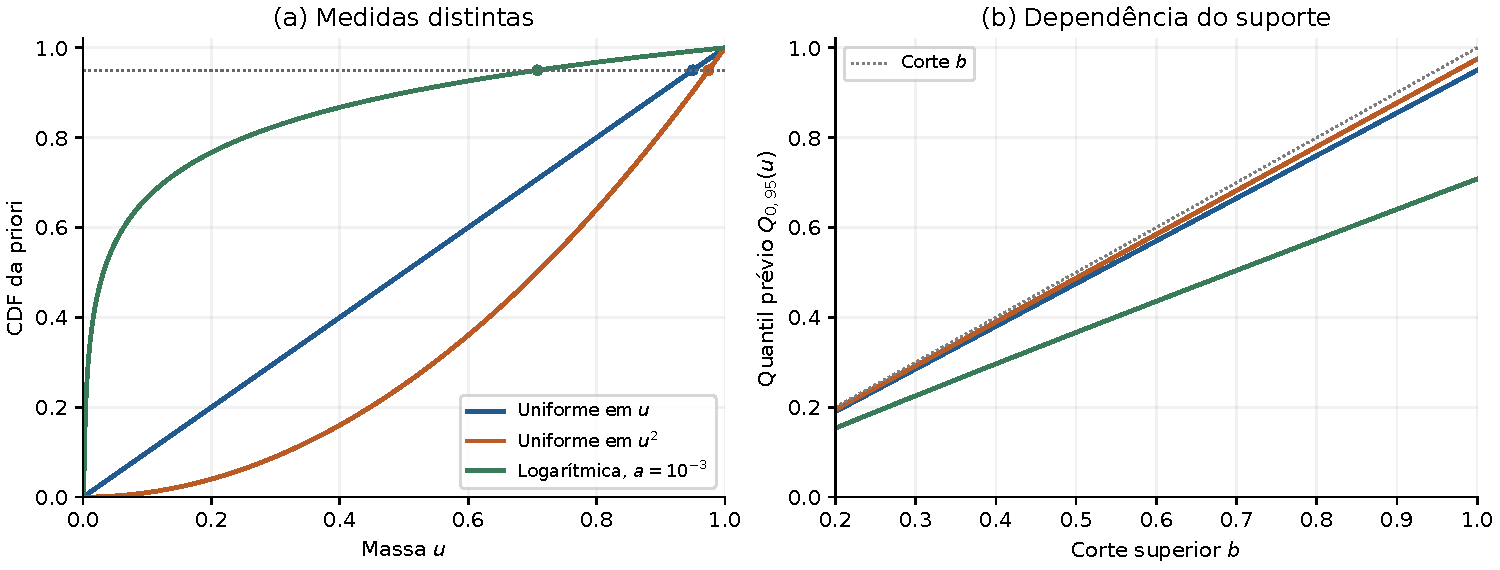
\includegraphics[width=\textwidth]{../figures/robustez/prioris_suporte.pdf}
 \caption{Referências analíticas de priori, sem dados simulados. À esquerda,
 as três CDFs e seus quantis de ordem \(0,95\): \(0,9500\), \(0,9747\) e
 \(0,7079\). As duas primeiras medidas têm suporte \([0,1]\); a logarítmica
 usa \([10^{-3},1]\). À direita, o corte superior \(b\) varia, mantendo
 corte inferior zero nas medidas uniformes e \(10^{-3}\) na logarítmica.
 Sob likelihood constante, essas curvas também são os quantis posteriores.}
 \label{fig:c09-prioris}
\end{figure}

Outro exemplo relevante para a comparação bibliográfica é a priori uniforme
 em velocidade de \textcite{wang2024graviton}. Para explicitar o
 Jacobiano na unidade adotada aqui, considere a conversão na frequência
 de referência \(1/T\). Se
 \(\beta\sim\mathcal U[\beta_{\min},1]\) e
 \(u=\sqrt{1-\beta^2}\), a medida induzida é
\begin{equation}
 \pi_u(u)=\frac{u}{(1-\beta_{\min})\sqrt{1-u^2}},\qquad
 0\leq u\leq\sqrt{1-\beta_{\min}^2}.
 \label{eq:c09-priori-velocidade}
\end{equation}
Ela difere das três medidas da Eq.~\eqref{eq:c09-prioris}. Por isso, comparar
limites publicados exige conservar também a transformação e o suporte da
priori, além da frequência usada para converter velocidade em massa.

Para um mesmo dado \(d\) e uma likelihood \(L(d\mid u)\), cada análise usa
\begin{equation}
 Z_\pi(d)=\int_a^b L(d\mid u)\pi(u)\,du,\qquad
 p_\pi(u\mid d)=\frac{L(d\mid u)\pi(u)}{Z_\pi(d)}.
 \label{eq:c09-evidencia-priori}
\end{equation}
O contraste entre prioris deve manter esse dado e a likelihood. Uma nova
simulação com outra semente muda simultaneamente a observação e não mede,
isoladamente, a sensibilidade à priori. Se \(\pi_1\) e \(\pi_0\) têm suporte
compatível, vale ainda
\begin{equation}
 \frac{Z_{\pi_1}(d)}{Z_{\pi_0}(d)}
 =\mathbb E_{p_{\pi_0}(u\mid d)}
       \left[\frac{\pi_1(u)}{\pi_0(u)}\right].
 \label{eq:c09-reponderacao}
\end{equation}
A identidade não garante eficiência numérica de reponderação. Se a nova
priori atribui probabilidade a uma região ausente no suporte de \(\pi_0\),
essa região precisa ser integrada separadamente. Uma mudança de corte ou
de priori tampouco transforma uma amostra de calibração anterior em verdades
sorteadas da nova medida.

A informação relativa à priori é medida, em nats, por
\begin{equation}
 D_{\mathrm{KL}}[p_\pi\Vert\pi]
 =\mathbb E_{p_\pi}[\log L(d\mid u)]-\log Z_\pi(d).
 \label{eq:c09-kl-priori}
\end{equation}
Essa quantidade é invariante sob uma mudança bijetiva de coordenada quando
as duas densidades recebem o mesmo Jacobiano. Ela muda quando se altera a
medida de priori. A igualdade de um único quantil posterior e prévio não
determina a divergência: redistribuições de massa dentro das regiões abaixo
e acima desse quantil podem manter sua posição e modificar a densidade.
Por isso, quantis, larguras, distâncias entre CDFs e divergência são produtos
distintos, cada um com seu controle numérico.

\section{Covariância e hipóteses de ruído}
\label{sec:c09-fatorial}

Para a estatística comprimida \(z\), as quatro variantes normais usam a
mesma média variável \(\mu(u)\). Elas combinam covariância completa ou
diagonal com covariância variável ou fixada em uma massa de referência
declarada. A densidade em cada variante é
\begin{equation}
 \log L=-\frac12\left[
 (z-\mu)^{\mathsf T}\Sigma^{-1}(z-\mu)
 +\log\det\Sigma+D\log(2\pi)\right].
 \label{eq:c09-normal-fatorial}
\end{equation}
O termo de determinante participa da comparação quando \(\Sigma\) varia.
Fixar a covariância não equivale a fixar a média. Nas observações físicas,
a densidade normal aplicada à estatística quadrática continua sendo uma
aproximação; sua aprovação numérica não a converte em distribuição exata.

Não existe ordenação universal da informação após diagonalizar uma
covariância. Considere o exemplo local
\(\Sigma=\left(\begin{smallmatrix}1&\rho\\\rho&1\end{smallmatrix}\right)\)
e uma média linear com derivada \(g\), com \(|\rho|<1\). Para
\(g=(1,1)^{\mathsf T}\), a informação de Fisher é
\(2/(1+\rho)\); para \(g=(1,-1)^{\mathsf T}\), é
\(2/(1-\rho)\). A substituição diagonal fornece \(2\) em ambos os casos.
Com \(\rho>0\), portanto, o sentido da alteração depende da direção do
sinal. Esse contraexemplo local fundamenta medir a direção do efeito sobre
os limites posteriores, sem tratá-la como propriedade universal.

\begin{figure}[htbp]
 \centering
 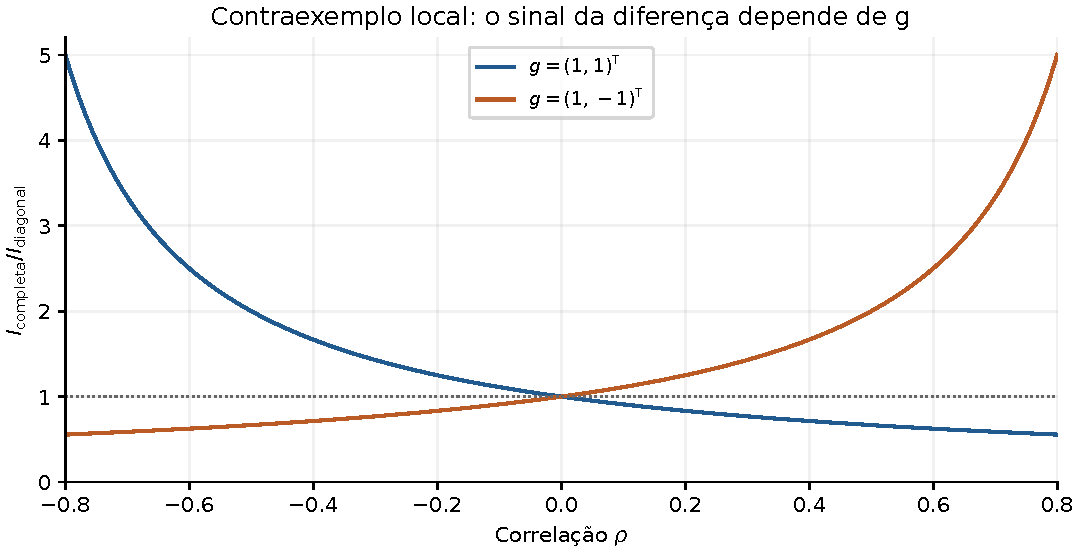
\includegraphics[width=0.88\textwidth]{../figures/robustez/fisher_direcao.pdf}
 \caption{Razão analítica entre as informações de Fisher completa e diagonal
 no exemplo de duas dimensões. A mesma correlação pode aumentar ou diminuir
 essa razão, conforme a derivada da média \(g\). Trata-se de um contraexemplo
 local, não de uma previsão quantitativa dos limites PTA.}
 \label{fig:c09-fisher-direcao}
\end{figure}

Uma hipótese discreta de distância com escalas \(s_j\) e probabilidades
\(w_j\) deve ser marginalizada na likelihood,
\begin{equation}
 L_{\mathrm{marg}}(d\mid u)=\sum_j w_j L(d\mid u,s_j),\qquad
 \sum_jw_j=1.
 \label{eq:c09-mistura-distancia}
\end{equation}
Em geral, essa mistura de densidades não é a densidade normal obtida ao
substituir suas covariâncias pela média. Uma escala global compartilhada
pelos pulsars também representa uma hipótese diferente de distâncias
astrométricas independentes.

\section{Interpretação da escala de massa}
\label{sec:c09-escala}

No suporte propagante adotado, \(u\leq1\) equivale a
\(m_gc^2\leq h/T\). Sob uma likelihood constante e priori uniforme em
\(u\), segue exatamente \(Q_{0,95}(m_gc^2)=0,95h/T\). Esse cálculo é uma
referência sem informação dos dados, e não uma previsão da posterior real.
Um limite numérico próximo dessa escala deve ser comparado com a priori,
a forma posterior e os controles de integração antes de se atribuir sua
origem à sensibilidade física. O contraste com a análise MeerKAT de
\textcite{zhao2026} permanece condicionado às diferenças de dados,
modelagem, parametrização e suporte; o experimento Fourier deste trabalho
não constitui uma reanálise de tempos de chegada observacionais.

% Texto sustentado pelos registros nominal14, D1 e D1b já executados.
\section{Validação separada das quantidades posteriores}
\label{sec:c09-validacao-funcional}

O cálculo de um quantil de massa e o de uma probabilidade ordenada pela
likelihood são problemas numéricos diferentes. Para uma verdade injetada
\(u_\star\), a probabilidade acumulada de massa é
\begin{equation}
 F(u_\star\mid d)=Z^{-1}\int_a^{u_\star}L(d\mid u)\pi(u)\,du.
 \label{eq:c09-pit-massa}
\end{equation}
Seu domínio tem fronteira conhecida. Já a quantidade dependente do dado
\begin{equation}
 H(d,u_\star)=Z^{-1}\int_{\{u:\,\log L(d\mid u)\leq
                  \log L(d\mid u_\star)\}}
                  L(d\mid u)\pi(u)\,du
 \label{eq:c09-pit-logl}
\end{equation}
exige identificar todas as componentes do conjunto integrado. Uma pequena
oscilação pode ter efeito reduzido na CDF de massa e introduzir vários
cruzamentos do nível de log-likelihood. Verificar alguns pontos ou apenas
o primeiro cruzamento não controla esse segundo cálculo.

Um exemplo analítico torna explícita a distinção. Para priori uniforme em
\([0,1]\) e \(L(u)=1+\varepsilon\sin(2\pi n u)\), com
\(0<\varepsilon<1\) e \(n\) inteiro positivo, tem-se \(Z=1\) e
\begin{equation}
 F(u)-u=\frac{\varepsilon}{2\pi n}
              [1-\cos(2\pi n u)].
 \label{eq:c09-exemplo-oscilatorio}
\end{equation}
Logo, \(\sup_u|F(u)-u|\leq\varepsilon/(\pi n)\), enquanto a amplitude
das oscilações de log-likelihood não diminui com \(n\). Esse exemplo não é
uma validação do modelo PTA: justifica controles próprios para cada
quantidade e a preservação de uma falha do evento de logL quando a CDF de
massa já está numericamente resolvida.

Para uma CDF referenciada, sejam \(N\) e \(Z\) os integrais não normalizados
do numerador e denominador, com estimativas de intervalo
\([N_-,N_+]\) e \([Z_-,Z_+]\), \(Z_->0\). A propagação usada é
\begin{equation}
 F\in\left[\max(0,N_-/Z_+),\;
                  \min(1,N_+/Z_-)\right].
 \label{eq:c09-razao-integral}
\end{equation}
Os erros de quadratura adaptativa são estimativas operacionais. A aritmética
de ponto flutuante empregada não fornece, por si só, limites rigorosos com
arredondamento dirigido. O termo ``intervalo operacional'' mantém essa
distinção em relação a uma demonstração uniforme do erro.

Um intervalo candidato \([u_-,u_+]\) para o quantil de ordem \(p\) só passa
no controle de referência quando sua largura é no máximo \(0,001\) e
\begin{equation}
 F_{\rm ref,+}(u_-)\leq p\leq F_{\rm ref,-}(u_+).
 \label{eq:c09-bracket-quantil}
\end{equation}
São exigidas também concordância entre resoluções e referências próprias:
\(0,001\) para log-evidência, momentos, KL e distância de Wasserstein em
\(u\), e \(0,002\) para CDF. Uma tolerância é um critério de aceitação;
não é uma medição de erro que possa ser somada como se tivesse sido observada.
O teste de cada métrica conserva seu alcance e suas possíveis falhas.


\subsection{Validação dos eventos e referências independentes}

A busca dos conjuntos de nível da verossimilhança classifica células como internas, externas ou ambíguas. Quando $N$ representa a integral das células internas e $A$ a contribuição ambígua, a propagação é
\begin{equation}
 H\in\left[\max(0,N_-/Z_+),\;\min(1,(N_++A_+)/Z_-)\right].
 \label{eq:c09-intervalo-evento}
\end{equation}
A subdivisão prioriza regiões com maior massa ambígua. Integrais independentes verificam as uniões de células e os extremos dos intervalos candidatos, sem pressupor um número fixo de cruzamentos.

Nos estudos preliminares, a concordância de CDFs de massa coexistiu com falhas do evento de log-verossimilhança. Em catorze casos fixos, treze eventos da representação tabulada atingiram o critério operacional, enquanto o caso de ruído vermelho forte permaneceu não resolvido. Esses casos não constituem calibração sob a priori nem demonstram precisão da resposta física entre todos os nós. Sua consequência metodológica foi exigir controles separados da resposta, da malha e das quantidades posteriores.

As comparações de prioris e covariâncias utilizam os mesmos dados para isolar a mudança de hipótese. Referências de quadratura verificam normalização, quantis, momentos, divergência de Kullback--Leibler e distância de Wasserstein. Nos modelos com mistura de distâncias, a integração sobre distância recebe refinamento próprio. A concordância de duas ordens é tratada como evidência finita, sem promover automaticamente referências adaptativas que não atingiram seus critérios de parada. Os resultados populacionais seguintes aplicam essas distinções e conservam os casos não resolvidos.

\section{Produção: robustez, informação e calibração condicional}
\label{sec:c09-producao}

A produção usa o experimento periódico de Fourier definido anteriormente,
com parâmetros auxiliares conhecidos. Foram geradas e verificadas
\(5\,396\) observações, analisadas em \(25\,956\) posteriores de base.
O painel pareado de prioris contém \(1\,600\) integrações sobre os mesmos
\(32\) dados centrais, dez análises e cinco medidas: \(320\) integrações
reavaliam a priori uniforme já existente e \(1\,280\) são contrastes
adicionais. Não são novas observações nem uma calibração SBC das prioris
reponderadas. As sementes, os identificadores, as configurações e os
resultados preservam também os casos numericamente indeterminados.

As tabelas positivas interpolam log-verossimilhança em
\(\alpha=\arcsin u\), por PCHIP, e integram dentro de cada intervalo por
quadratura positiva. Malhas aninhadas, ordens 32 e 16 e referências
independentes selecionadas verificam os funcionais. A concordância nesses
testes tem alcance finito: não constitui limite uniforme de erro da
resposta física. Na síntese dos quantis, uma análise sem aprovação dos
critérios de malha e resposta recebe \([0,1]\); nenhum ID é eliminado.
Os intervalos descritivos deste capítulo propagam a incerteza numérica,
não a incerteza amostral de uma média populacional.

\subsection{Sensibilidade à medida e ao suporte}

No painel de mesmos dados, a mediana de \(Q_{0,95}\) de A0 é
\([0,9355;0,9360]\) para a priori uniforme em \(u\),
\([0,9670;0,9675]\) para a uniforme em \(u^2\) e
\([0,6856;0,6861]\) para a logarítmica com corte \(10^{-3}\).
Alterar apenas esse corte para \(10^{-4}\) ou \(10^{-2}\) fornece,
respectivamente, \([0,6184;0,6189]\) e \([0,7663;0,7668]\).
As medianas de KL correspondentes ficam entre \(0,0261\) e
\(0,0489\) nat. A proximidade de alguns quantis aos quantis prévios
é acompanhada por medidas de informação; não é tomada isoladamente como
prova de ausência de aprendizado.

Para B construído das observações CN, com covariância completa e variável,
a priori uniforme produz mediana de \(Q_{0,95}\) em
\([0,9473;0,9478]\) e KL mediana de \(0,00230\) nat. Com corte
logarítmico \(10^{-4}\), os valores são \([0,6165;0,6170]\) e
\(0,00166\) nat. Assim, neste experimento condicional e neste painel,
a escolha de medida e suporte altera o limite muito mais que a pequena
distância informacional típica da posterior comprimida à sua própria
priori. Isso não estabelece um teorema de ausência de informação em PTAs.
W1, diferenças de CDF e razões de odds para \(u\leq0,2\) estão também
registrados por dado; a interpretação não depende de um único quantil.

\subsection{Fatorial da covariância}

O desenho separa covariância completa/diagonal de fixa/variável e conserva
o termo log-determinante da densidade normalizada. São \(24\) contrastes
de \(500\) pares, cobrindo três prioris e as duas origens de observações B.
Para B de origem CN e priori uniforme, diagonal menos completa, ambas
variáveis, tem diferença média de \(Q_{0,95}\) em
\([-0,00047;0,00051]\). Há \(17\) pares com diferença negativa,
\(14\) positiva e \(469\) com sinal não resolvido numericamente.
Com priori logarítmica, esses números são \(175\), \(174\) e \(151\).
A diagonalização pode produzir efeitos de ambos os sinais; não é
universalmente conservadora. Médias compatíveis com zero na resolução
usada não demonstram equivalência entre os procedimentos.

A escolha fixa/variável é um eixo distinto. No mesmo B de origem CN,
com priori uniforme e matriz completa, fixa menos variável apresenta
média em \([0,00020;0,00118]\). Em B de origem gaussiana com priori
logarítmica, a média correspondente é negativa,
\([-0,00133;-0,00036]\). São descrições das realizações registradas,
sem intervalo de confiança populacional ou extrapolação a outros sinais.

\subsection{Contaminantes: limites mais baixos podem ser incorretos}

Quatro cenários usam \(64\) realizações em \(u_*=0,5\), com
contaminante monopolar ou dipolar de amplitude relativa \(0,25\) ou \(1\).
A comparação pareada conserva a observação e omite ou inclui o componente
conhecido na covariância. A Tabela~\ref{tab:c09-contaminantes-producao}
apresenta os contrastes de A0; os \(12\) contrastes completos abrangem
também as duas análises B.

\begin{table}[htbp]
\centering
\caption{Média descritiva de \(\Delta Q_{0,95}\), omissão menos inclusão,
em A0. Intervalos numéricos; \(64\) pares por linha.}
\label{tab:c09-contaminantes-producao}
\begin{tabular}{lcc}
\hline
Componente & Amplitude relativa & Intervalo da média\\
\hline
Monopolar & \(0,25\) & \([-0,06715;-0,06617]\)\\
Monopolar & \(1\) & \([-0,18319;-0,18221]\)\\
Dipolar & \(0,25\) & \([-0,04852;-0,04754]\)\\
Dipolar & \(1\) & \([-0,30819;-0,30721]\)\\
\hline
\end{tabular}
\end{table}

No cenário dipolar de amplitude relativa unitária, A0 apresenta mediana
de quantil \([0,9504;0,9509]\) com inclusão e
\([0,6655;0,6660]\) com omissão. Em \(61\) dos \(64\) pares o
quantil diminui com sinal resolvido. Um limite aparentemente mais forte
pode, portanto, decorrer de especificação incorreta. Em B de origem CN,
a diferença média nesse cenário é \([-0,01264;-0,01167]\): a resposta
menor à omissão também não demonstra robustez observacional, especialmente
quando a compressão já retém pouca informação sobre a massa.

\subsection{Ruído, espectro e variabilidade entre realizações}

Os dois cenários de ruído contêm \(500\) realizações cada. Em A0, as
medianas de KL são \(0,01121\) nat sob ruído vermelho forte e
\(0,01920\) nat sob ruído branco forte. Em B de origem CN são
\(0,00284\) e \(0,00042\) nat. As medianas dos quantis ficam próximas
de \(0,95\), mas os percentis entre realizações e as KL distinguem
as distribuições. As realizações de cenários diferentes têm sementes
próprias; diferenças entre essas medianas não são contrastes pareados.

Nos cenários espectrais, com \(64\) realizações por combinação de inclinação
e massa fixa, o expoente \(3\) fornece KL mediana de A0 de
\(0,00752\) nat em \(u_*=0,5\). Com expoente \(5,5\), ela passa a
\(0,09961\) nat; a mediana de \(Q_{0,95}\) passa de aproximadamente
\(0,9502\) a \(0,9141\). Perto do corte, \(u_*=0,995\), o espectro
\(5,5\) fornece KL mediana \(0,26076\) nat e quantil mediano
\([0,9751;0,9756]\). Não se aplica a hipótese uniforme de SBC a esses
cenários de massa fixa. Os \(128\) dados por massa do painel de fronteiras
completam a descrição da variabilidade condicional.

\subsection{Distâncias e indeterminação numérica}

O cenário de distâncias sorteia uma escala global entre \(0,9\), \(1\)
e \(1,1\), com pesos \(0,25\), \(0,50\) e \(0,25\). A inferência
correta soma as densidades completas, após todos os canais; não mistura
covariâncias nem sorteia uma escala independente por frequência. Compara-se
essa mistura à análise com escala nominal sobre os mesmos \(500\) dados.

As \(3\,000\) posteriores foram integradas, mas \(834\) análises A0
falharam no controle pontual de interpolação da resposta em logL.
Preservando esses casos como quantis \([0,1]\), o contraste médio
nominal menos mistura em A0 fica em \([-0,90362;0,76454]\), inconclusivo.
Nas duas análises B, os \(500\) contrastes têm sinal não resolvido e
média em cerca de \([-0,00049;0,00049]\). A resolução adotada não permite
afirmar equivalência, nem que incertezas de distância sejam irrelevantes.

\subsection{Calibração da massa e dos eventos de likelihood}

A família prospectiva contém \(18\) grupos de \(500\) observações e
\(126\) testes. Foram conservados todos os IDs, inclusive os intervalos
indeterminados \([0,1]\). No conjunto de \(9\,000\) análises SBC,
\(8\,621\) PIT de massa e \(8\,179\) PIT de logL têm resolução
operacional. Os eventos usam o limiar avaliado diretamente na resposta
física da massa verdadeira. As regiões desconectadas são integradas na
tabela positiva; patamares seriam tratados separadamente como átomos.
Nenhum átomo foi encontrado nos interpolantes desta produção.

A troca do limiar interpolado pelo físico é relevante: uma diferença de
logL de apenas \(1,2091\times10^{-5}\) alterou uma probabilidade de evento
em \(0,139777\). Assim, uma tolerância pontual de logL não é, sozinha,
um limite de erro para a probabilidade do evento. Após os controles de
discretização, de resposta e de limiar, a família completa com correção de
Holm a \(0,05\) apresenta \(116\) não rejeições para todos os valores
admissíveis dos intervalos fornecidos e \(10\) testes numericamente
indeterminados. Não há rejeição robusta nesta síntese condicional.
Os envelopes observados não possuem certificado físico uniforme:
não rejeitar não prova calibração física completa, aprendizado da massa
ou equivalência entre modelos. Os registros da síntese preliminar sem
eventos permanecem preservados como histórico.

\subsection{Escala física e alcance das conclusões}

Como \(m_gc^2=(h/T)u\), todo quantil relatado neste experimento é
\(Q_{0,95}(m_gc^2)=(h/T)Q_{0,95}(u)\). Sob priori uniforme e likelihood
constante, ele já vale \(0,95h/T\). Portanto, proximidade de um limite
à escala \(h/T\), como no benchmark MeerKAT discutido na revisão, precisa
ser interpretada com a medida, o suporte, as frequências e o modelo
probabilístico completos. Os resultados do painel de prioris ilustram
quantitativamente esse problema, sem reanalisar as observações MeerKAT.

Os dados sintéticos periódicos não incorporam automaticamente cadência
irregular, ajuste do modelo de temporização, acoplamento entre frequências
ou possível impropriedade complexa dos coeficientes obtidos de TOAs reais.
Também não marginalizam os parâmetros auxiliares aqui conhecidos.
Comparações de evidência entre espaços de observação diferentes não são
interpretadas como fatores de Bayes. A extensão escalar e a aproximação
observacional permanecem tarefas próprias de C10 e C11.

A consolidação está em \path{results/C09/robustness_synthesis/}, com
\(90\) grupos descritivos, \(39\) contrastes e \(14\,268\) diferenças
pareadas. O acumulado C09 é de \(67\,072\,009\) avaliações de likelihood;
o acumulado físico D3 é de \(7\,920\) nós e aproximadamente
\(85,696\) trilhões de produtos reais estimados. Falhas e tentativas
interrompidas permanecem contabilizadas. Foram restaurados e conferidos
\(24\,238\) arquivos lógicos a partir dos pacotes da produção e de suas
dependências. O manifesto da versão vincula fontes, resultados e PDF.

